\documentclass[polish, 11pt]{article}

\usepackage[a4paper,
  top=.5cm,
  bottom=2.5cm,
  left=2.5cm,
  right=2.5cm,
  headheight=86pt, % as per the warning by fancyhdr
  includehead,includefoot,
  heightrounded, % to avoid spurious underfull messages
]{geometry}
\usepackage{babel}
\usepackage{polski}
\usepackage[utf8]{inputenc}
\usepackage[T1]{fontenc}
\usepackage{graphicx}
\usepackage{float}
\usepackage{minted} % na razie zostawiłem ale do pseudokodu minted chyba nie ma wsparcia - jest coś jak algorithm2e ale nie przyglądałem sie bardziej albo po prostu listings
\usemintedstyle{xcode}
\usepackage{booktabs}
\usepackage{multirow}
\usepackage{listings}
\lstset{
  basicstyle=\ttfamily,
  columns=fullflexible,
  frame=single,
  breaklines=true,
  postbreak=\mbox{\textcolor{red}{$\hookrightarrow$}\space},
}

\usepackage{fancyhdr}
\pagestyle{fancy}
\fancyhf{}
\fancyheadoffset[L]{2cm}
\lhead{
\includegraphics[height=2cm]{figures/PWRlogo.jpg}\\
    \vspace{3mm}
    Tytuł projektu: Apapp
    \vspace{1mm}
}
\cfoot{Wrocław, 2019}
\rfoot{\thepage}

\begin{document}
{
    \centering
    \Huge{PROJEKTOWANIE SYSTEMÓW INTERNETOWYCH I MOBILNYCH}
\vspace{2cm}

    \huge{WYDZIAŁ ELEKTRONIKI - INFORMATYKA \\ Systemy i Sieci Komputerowe}
\vspace{2cm}

    \LARGE{\textbf{Tytuł projektu: Apapp}}
\vspace{3cm}

    \begin{flushright}
        Zespół projektowy:\\
        Janusz Długosz, 235746\\
        Jakub Dorda, 235013\\
        Marcin Kotas, 235098\\
        Mateusz Polok, 234981
        
    \end{flushright}
}
\newpage
\tableofcontents
\newpage

\section{Cel i zakres projektu}
    Tematem projektu została aplikacja mobilna „TrueHome”, która na celu ma wykorzystać lukę na rynku ogłoszeń oferujących wynajem mieszkania. Luka ma postać braku możliwości oceny osoby wynajmującej oraz najmującej mieszkanie, co wydłuża proces znalezienia odpowiedniej osoby w zależności od sytuacji.
    
    \subsection{Minimal Viable Product}
        \begin{enumerate}
            \item \textbf{Moderator}
            \begin{itemize}
                \item ma możliwość usuwania ofert
                \item ma możliwość usuwania użytkowników
                \item dostaje powiadomienia o naruszeniach regulaminu aplikacji
            \end{itemize}
            
            \item \textbf{Zwykły użytkownik}
            \begin{itemize}
                \item szuka mieszkania
                \item ma możliwość wyboru lokalizacji, w której szukam mieszkania (miasto, promień)
                
                \item ma możliwość filtracji listy mieszkań:
                \begin{itemize}
                    \item Cena
                    \item Pokój iloosobowy
                    \item Ilość osób w mieszkaniu
                \end{itemize}
                
                \item ma możliwość zobaczenia szczegółów mieszkania:
                \begin{itemize}
                    \item Zdjęcia
                    \item Adres
                    \item Cena
                    \item Ilość osób w mieszkaniu
                    \item Numer kontaktowy lub mail do właściciela
                \end{itemize}
                
                \item ma możliwość oceny mieszkania po potwierdzeniu wynajęcia przez użytkownika będącego  właścicielem mieszkania
                \item ma możliwość zgłoszenia naruszeń regulaminu aplikacji
            \end{itemize}
            
            \item \textbf{Użytkownik właściciel mieszkania}
            \begin{itemize}
                \item ma możliwość dodania mieszkania do wynajęcia
                \item ma możliwość zakończenia oferty
                \item ma możliwość potwierdzenia osoby najmującej (zwykły użytkownik)
                \item wybiera unikalną lokalizację za pomocą zewnętrznego API (np. Google Maps, OpenStreetMap)
            \end{itemize}
        \end{enumerate}
        
\section{Technologie informatyczne wykorzystane w projekcie}
    \subsection{Serwer}
        Serwer uruchamiany jest w dockerze na maszynie wirtualnej w serwisie DigitalOcean.
        Do zaprojektowania serwera REST wykorzystano technologię ASP.NET Core w wersji 2.1.
        Jako narzędzie pomocnicze przy wywoływaniu zapytań do bazy danych wykorzystano biblioteki Npgsql (połączenie z bazą) oraz Dapper (konstrukcja zapytań).
        Rejestrowanie błędów oraz komunikatów odbywa się za pomocą biblioteki NLog, która umożliwia wysoce konfigurowalne zapisywanie logów do konsoli oraz plików.
        Dodano również automatyczne generowanie dokumentacji dostępnego API za pomocą Swaggera (OpenAPI).
            
        Do uwierzytelniania i autoryzacji wykorzystano bibliotekę OpenIddict, która implementuje standard OpenID Connect.
        Do opisu danych kont użytkowników oraz obsługi zastosowano ASP.NET Core Identity.
        Wykorzystany został również Entity Framework Core zapewniający translację danych pomiędzy relacyjną bazą danych, a obiektami w programie (O/R mapping).
        
        Jako system zarządzający bazą danych wybrano PostgreSQL.
        
    \subsection{Android}
    	Aplikacja mobilna pisana jest w języku programowania Kotlin
    	Komunikację z REST api zapewniają popularne biblioteki Retrofit2 oraz OkHttp3 rozwijane przez firmę Square.
    	Parsowanie jsonów odbywa się przy pomocy biblioteki Gson.
    	
    	Ważnym elementem architektury aplikacji jest programowania reaktywne, w tym celu użyto implementacji Reactive Components znanych jako rodzina bibliotek ReactiveX w wersji RxKotlin. Dodatkowo wykorzystywane też są wtyczki RxAndroid do synchronizacji wątków systemowych oraz retrofit2:adapter-rxjava2 zapewniającej integrację ReactiveX z Retriofit2, umożliwia to obserwowanie zapytań sieciowych. Innym reaktywnym elementem architektury jest LiveData z Android Architecture Components, będący implementacją wzorca obserwator rozszerzonego o świadomość cyklu życia aplikacji Androidowej.
    	
    	Czystą architekturę oraz testowalność zapewnia stosowanie Dependency Injection na frameworku Dagger2.
    	
    	Komponenty widoku nie będące częścią podstawowych bibliotek pochodzą z rodziny AndroidX będącą następcą Android Support Libs.
    	
    	Dodatkowo w aplikacji w konfiguracji Debug wykorzystywany jest framework LeakCanary umożliwiający śledzenie i rozwiązywanie wycieków pamięci JVM. 

\section{Harmonogram prac projektowych – wykres Gantta}
    \begin{figure}[H]
        \centering
        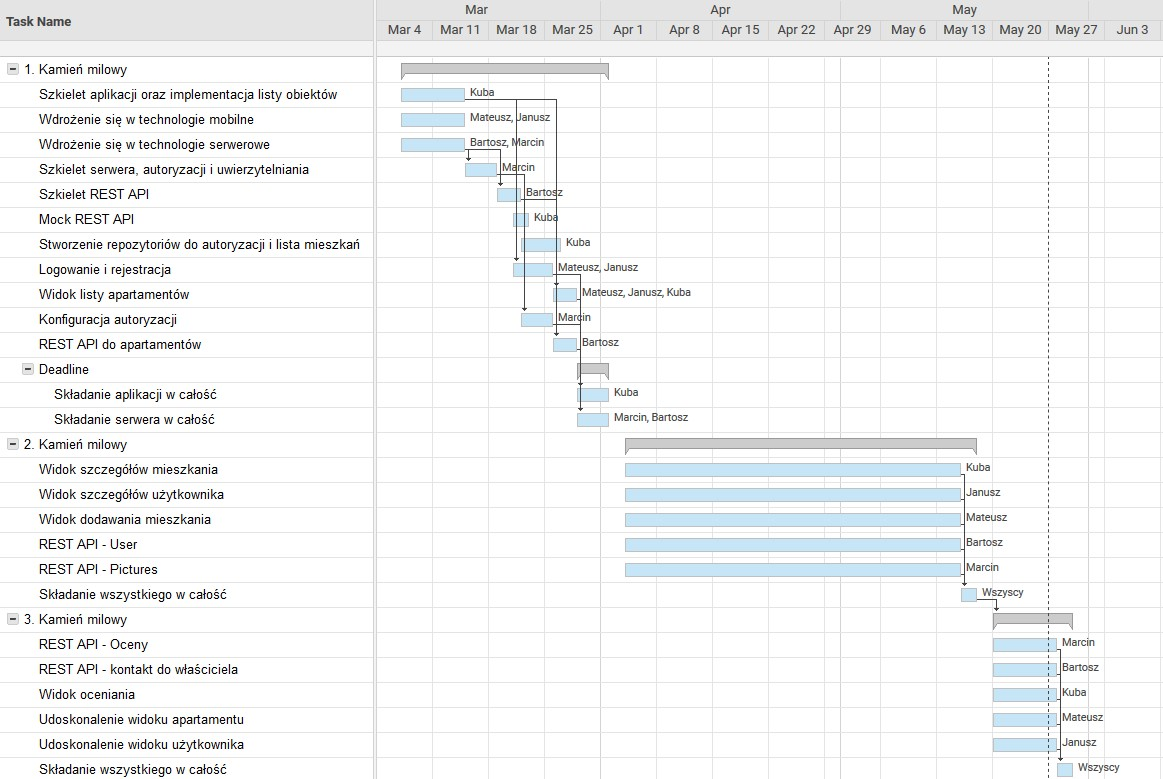
\includegraphics[width=\textwidth]{figures/gantt.jpg}
        \caption{Wykres Gantta}
    \end{figure}
    
\section{Architektura aplikacji}
    \begin{figure}[H]
        \centering
        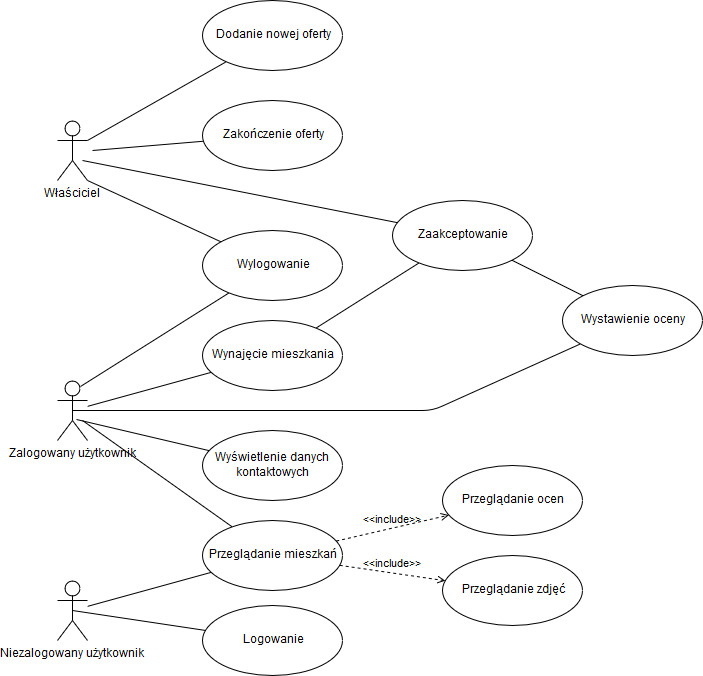
\includegraphics[width=\textwidth]{figures/UseCase.jpg}
        \caption{Diagram przypadków użycia}
    \end{figure}
    
    \subsection{Serwer}
        Utworzone zostały trzy kontenery:
        \begin{itemize}
            \item \textbf{ResourceServer} - główny serwer obsługujący zapytania REST.\\
            
            \item \textbf{AuthServer} - serwer pomocniczy służący do uwierzytelniania i autoryzacji użytkowników.\\
            
            \item \textbf{PostgresDB} - kontener zawierający bazę danych.\\
        
        \end{itemize}
        
        
        \begin{figure}[H]
            \centering
            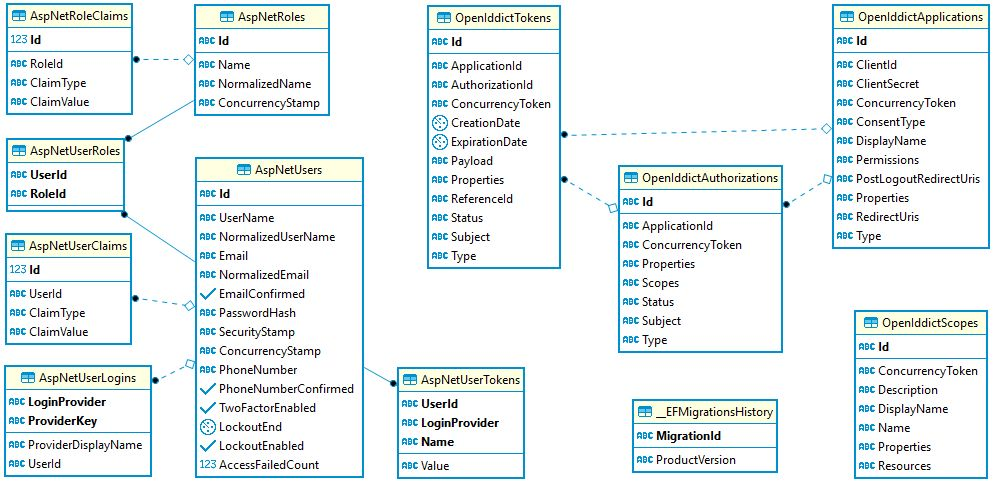
\includegraphics[width=\textwidth]{figures/AuthERD.jpg}
            \caption{Diagram ERD bazy autoryzacji}
        \end{figure}
        
        \begin{figure}[H]
            \centering
            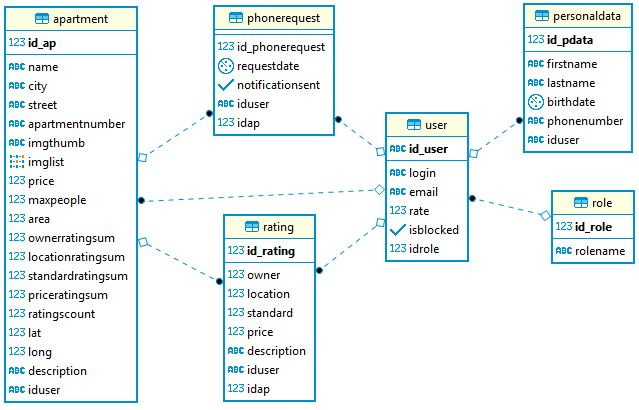
\includegraphics[width=\textwidth]{figures/TrueHomeERD.jpg}
            \caption{Diagram ERD głównej bazy aplikacji}
        \end{figure}
        
        \begin{figure}[H]
            \centering
            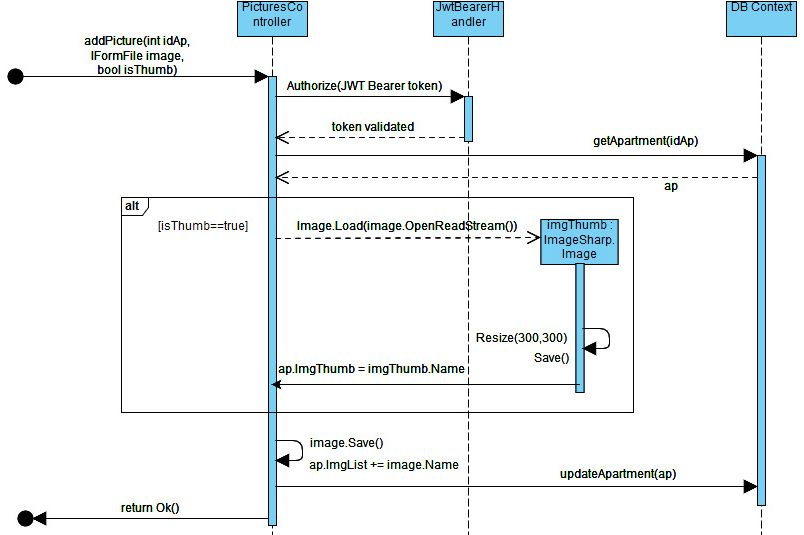
\includegraphics[width=\textwidth]{figures/addPictureSeq.jpg}
            \caption{Diagram sekwencji dodawania zdjęcia}
        \end{figure}
        
        \begin{figure}[H]
            \centering
            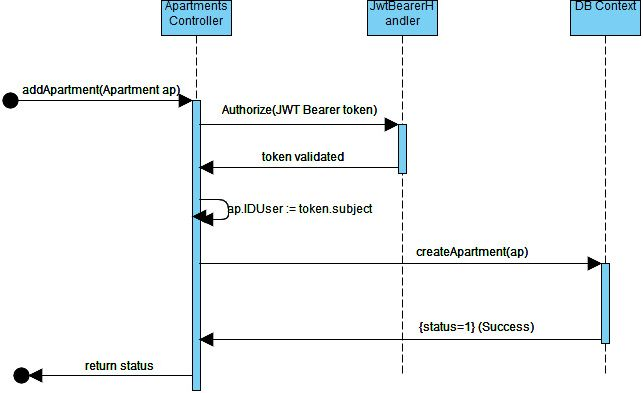
\includegraphics[width=\textwidth]{figures/addApartmentSeq.jpg}
            \caption{Diagram sekwencji dodawania apartamentu}
        \end{figure}
        
        \begin{figure}[H]
            \centering
            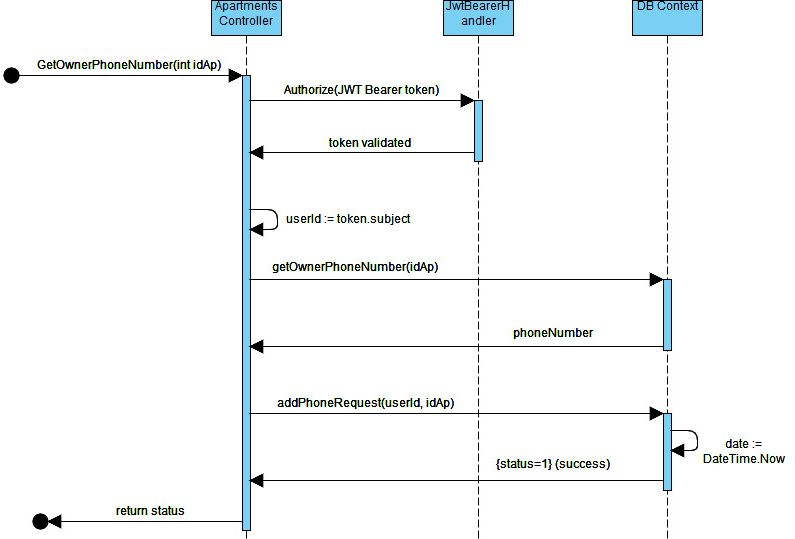
\includegraphics[width=\textwidth]{figures/getPhoneSeq.jpg}
            \caption{Diagram sekwencji pobierania numeru telefonu właściciela}
        \end{figure}
    
    \subsection{Android}
    
    Pierwszą warstwą aplikacji mobilnej jest komunikacja sieciowa z REST API. Zapytania sieciowe wykonywane są asynchronicznie z warstwy repozytoriów danych. Repozytoria wykorzystywane są do lokalnego cachowania oraz umożliwiają dostęp do tych samych danych z kilku różnych miejsc kolejnej warstwy abstrakcji. W zależności od potrzeb przy pomocy Dependency Injection repozytorium może być traktowane jako jedno lub wielo-instancyjne. Interfejs publiczny repozytoriów został zbudowany bazując na paradygmacie programowania reaktywnego, implementacja udostępnia obserwowalny, dyskretny potok danych zaimplementowany przy pomocy wzorca projektowego Behaviour Subject (wielu obserwatorów, jeden strumień, dostęp do wartości wyemitowanych w czasie t+1 po subskrypcji obserwatora). Z repozytoriów korzysta bezpośrednio warstwa ViewModelów. ViewModele odpowiadają za definiowanie zachowania widoków aplikacji oraz zapewniają dostęp do danych otrzymywanych z repozytoriów.
    ViewModele komunikują się z warstwą widoku (Fragmenty) przy pomocy LiveData będącego częścią biblioteki Android Architecture Components. LiveData jest implementacją wzorca Obserwator z dodatkową świadomością cyklu życia Fragmentu lub innego komponentu widoku do którego przypisany jest obserwator zmiennej LiveData. W uproszczeniu polega to na automatycznej subskrypcji oraz jej usunięciu w zależności czy dany widok aplikacji jest obecnie widoczny dla użytkownika. Umożliwia to dość znaczącą optymalizację, szczególnie w związku z tym, że z niższych warstw nowe wartości otrzymywane są asynchronicznie. Opcjonalną warstwą między ViewModelem a widokiem jest warstwa Data Bindingu, umożliwiająca obsługę modelu danych od razu w kodzie xml. Rozwiązanie to stosowane jest głównie w niezbyt skomplikowanych widokach nie wymagających interaktywności np. listach.
    
    \begin{figure}[H]
    	\centering
    	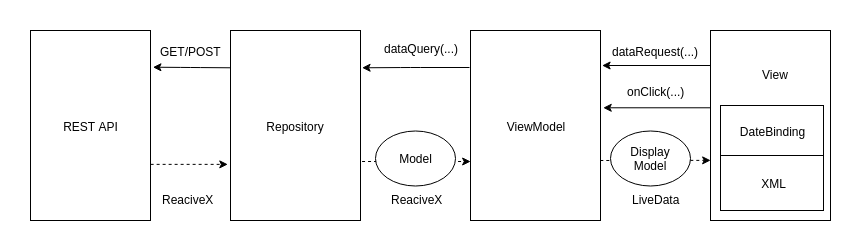
\includegraphics[width=\textwidth]{figures/androidArch.png}
    	\caption{Uproszczony schemat ideowy architektury aplikacji Androidowej}
    \end{figure}     
        
\section{Opis struktury kodowania aplikacji} %mateusz
    \subsection{handleNewLoginRequestStatus(status)}
        \begin{lstlisting}
        when (status) 
           Idle -> {}
           Pending -> 
                loginButton <- GONE
                registerButton <- GONE
                login_progress <- VISIBLE
                login_progress.progress <- 0
            Success -> 
                Toast(singed_in)
                switchToApartmentListFragment()
            BadCardinals -> 
                Toast(invalid_login_toast)
                loginButton <- VISIBLE
                registerButton <- VISIBLE
                login_progress <- GONE
            Error -> 
                Toast(login_error_toast)
                loginButton <- VISIBLE
                registerButton <- VISIBLE
                login_progress. <- GONE
         \end{lstlisting}
         Funkcja definiuje działania, które następują po próbie logowania. Ustawia widoczność przycisków w zależności od statusu. Jeśli logowanie nie powiedzie się to wyświetlony zostaje odpowiedni komunikat. Jeśli zaś wszystko pójdzie dobrze to funkcja przenosi użytkownika do kolejnego widoku (zawierającego listę dostepnych apartamentów).
    \subsection{addApartment(name, city, street, apartmentNumber, price, maxPeople, area, phoneNumber, lat, long)}
        \begin{lstlisting}
            rxDisposables.add(bearerAuthWrapper.wrapCall(
            bearerAuthWrapper.apiAuthService.addApartment(ApartmentAdd(name, city, street, apartmentNumber, price,
                maxPeople, area, phoneNumber, lat, long)))
                .observeOn(rxSchedulersFacade.io())
                .subscribeOn(rxSchedulersFacade.io())
                .subscribe({ t -> if(t!=null) apartmentIdSubject.onNext(t)},
                    { e -> Log(e, "ERROR adding Apartment") })
        \end{lstlisting}
        Funkcja wykorzystuje bibliotekę ,,Reactivex'' do asynchronicznego wysyłania strumieni danych dla nowo dodanej oferty mieszkania. Odbywa się to na osobnym wątku. Jeśli wystąpi błąd to stosowna informacja pojawi się w logach.
    \subsection{validatePassword(password, isPassword)}
         \begin{lstlisting}
        upperCasePattern <- [A-Z]
        digitCasePattern <- [0-9]
        if(isPassword)
            isPasswordCorrect <- false
        else 
            isRePasswordCorrect <- false
        registerPossibility <- (isEmailCorrect && isPasswordCorrect && isRePasswordCorrect
                && isLoginCorrect && isNameNotEmpty && isSurnameNotEmpty)
        if(!upperCase.find(password))
            if(isPassword)
                passwordStatus <- UPPERCASE
             else
                rePasswordStatus <- UPPERCASE
            return
        if(!digitCase.find(password))
            if(isPassword)
                passwordStatus.postValue <- DIGITCASE
             else
                rePasswordStatus.postValue <- DIGITCASE
            return
        if(password.length < 8)
            if(isPassword)
                passwordStatus <- LENGTH
            else
                rePasswordStatus <- LENGTH
            return
        if(isPassword)
            isPasswordCorrect <- true
            passwordStatus <- OK
        else 
            isRePasswordCorrect <- true
            rePasswordStatus <- OK
        
        registerPossibility <- (isEmailCorrect && isPasswordCorrect && isRePasswordCorrect
                && isLoginCorrect && isNameNotEmpty && isSurnameNotEmpty)
         \end{lstlisting}
         Funkcja sprawdza kolejno czy podane przez użytkownika hasło spełnia wymogi. Konkretnie sprawdzane jest czy hasło zawiera co najmniej po jednej dużej literze i cyfrze, a oprócz tego sprawdza czy długość wynosi co najmniej 8. Jeśli wszystkie warunki są spełnione to w zmiennej \texttt{registerPossibility} zapisana jest możliwość zarejestrowania się w aplikacji, która zostanie wykorzystana w innej funkcji.  
    \subsection{onNewAuthStatus(status)}
        \begin{lstlisting}
            when(status)
                IDLE -> {}
                LOGGED_IN -> {}
                NO_INTERNET ->  Toast(no_internet)
                REQUEST_FAILED -> Toast(no_api_response)
                LOGOUT_USER -> logout()
                LOGOUT_FORCED -> 
                    logout()
                    Toast(session_expired_toast)
              
            
        \end{lstlisting}
        Funkcja po otrzymaniu odpowiedzi w procesie uwierzytelnienia decyduje, co dalej robić. W razie niepowodzenia wyświetla odpowiednie komunikaty. Dzięki niej jest możliwe wylogowanie się z aplikacji.

\section{Prezentacja aplikacji}

    \subsection{Logowanie}
        \begin{figure}[H]
                    \centering
                    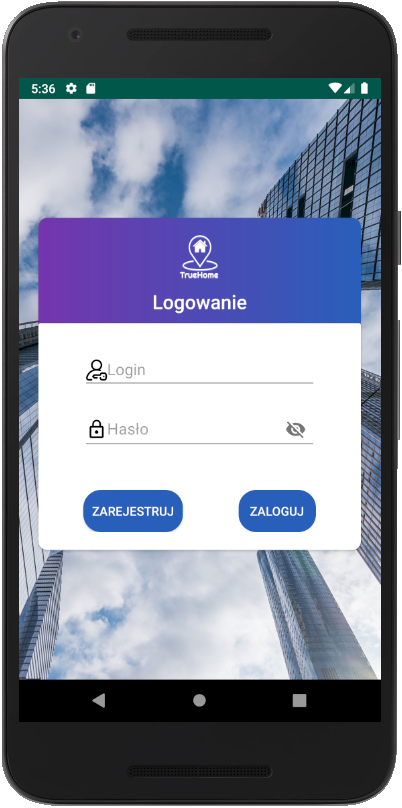
\includegraphics[width=0.45\textwidth]{aplikacja/logowanie.png}
                    \caption{Panel logowania}
        \end{figure}
        
         W tym miejscu po podaniu prawidłowego loginu i hasła oraz naciśnięciu \texttt{ZALOGUJ} można wejść do głównego panelu, czyli przeglądania dostępnych mieszkań. Jeśli użytkownik nie ma konta w aplikacji to może nacisnąć \texttt{ZAREJESTRUJ} i przejść do procesu rejestracji. Jeśli logowanie się powiedzie to przy następnym uruchomieniu ,,TrueHome'' aplikacja przejdzie od razu do panelu głównego.
    \subsection{Rejestracja}
        \begin{figure}[H]
                    \centering
                    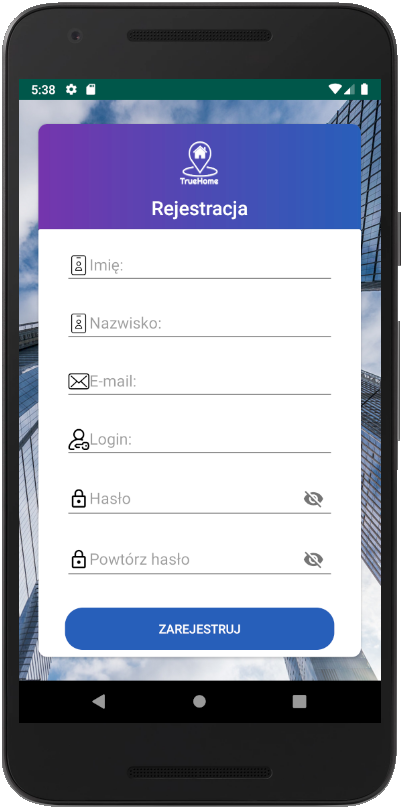
\includegraphics[width=0.45\textwidth]{aplikacja/rejestracja.png}
                    \caption{Panel rejestracji}
        \end{figure}
        
        Aby móc się zarejestrować w aplikacji należy uzupełnić wszystkie rubryki swoimi danymi, tj. imię, nazwisko, e-mail, login, hasło. Podczas wpisywania  e-mail weryfikowana jest poprawność wprowadzonego adresu. Podobnie przy wpisywaniu hasła sprawdzane jest czy spełnia ono wszystkie warunki, czyli posiada po co najmniej jednej wielkiej literze i jednej cyfrze oraz co najmniej 8 znaków w sumie. Jeśli te dane nie zostaną poprawnie wprowadzone lub jeśli hasło zostanie źle powtórzone to rejestracja się nie powiedzie. Po poprawnym wypełnieniu wszystkich rubryk należy wcisnąć \texttt{ZAREJESTRUJ}, wówczas dostaniemy odpowiedź czy proces się powiódł. Jeśli z jakiegoś względu użytkownik zechce zaniechać rejestracji to musi wcisnąć systemowy przycisk powrotu. W aplikacji nie występuje podział kont na osoby wystawiające mieszkania oraz wynajmujące, każdy zarejestrowany posiada pełną funkcjonalność.
     \subsection{Przeglądanie mieszkań}
        \begin{figure}[H]
                    \centering
                    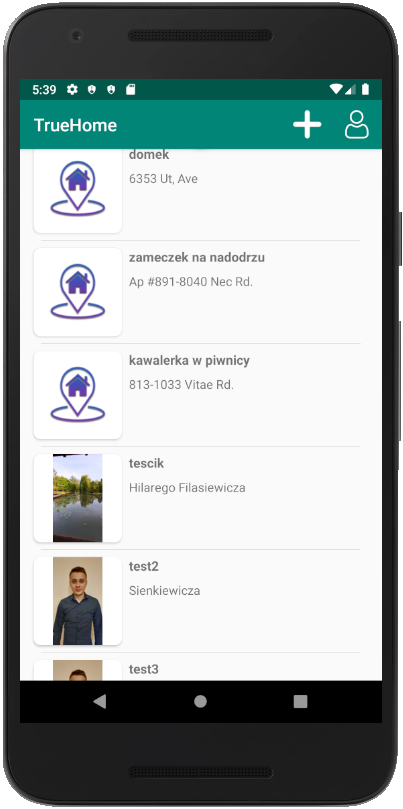
\includegraphics[width=0.45\textwidth]{aplikacja/main.png}
                    \caption{Panel przeglądania mieszkań}
        \end{figure}
        
       Jest to główny panel ,,TrueHome''. Tutaj można przeglądać aktualne oferty mieszkań do wynajęcia. Listę można przewijać oraz odświeżać. W prawym górnym rogu znajdują się kolejno przyciski przenoszące do ,,Dodawania oferty'' oraz do ,,Panelu użytkownika'' Po wciśnięciu przez użytkownika interesującej go oferty, zostanie przeniesiony do szczegółów. Jeśli pobieranie listy mieszkań się nie powiedzie to zostanie wyświetlony stosowny komunikat.
      \subsection{Szczegóły użytkownika}
        \begin{figure}[H]
                    \centering
                    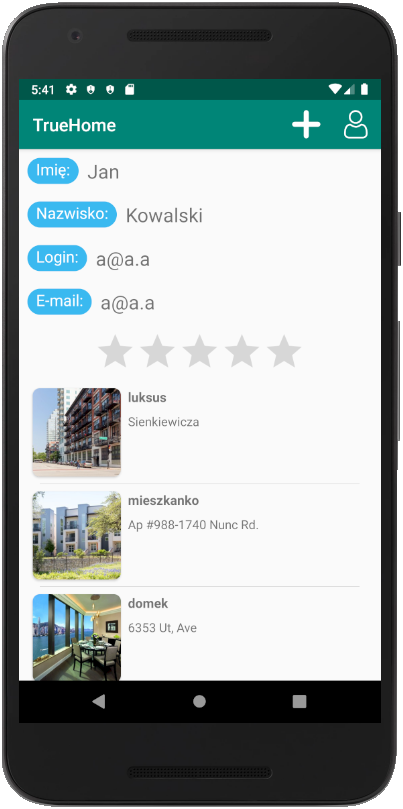
\includegraphics[width=0.45\textwidth]{aplikacja/user_panel.png}
                    \caption{Panel użytkownika}
        \end{figure}
        
        W tej zakładce użytkownik ma możliwość sprawdzenia swoich najważniejszych danych, tj. imię, nazwisko, login, adres e-mail, na które zostało założone konto oraz jego średnią ocen wystawionych przez użytkowników wynajmujących mieszkania. Poniżej tych informacji znajduje się lista mieszkań wystawionych przez osobę aktualnie zalogowaną. Można ją przewijać i odświeżać, a po naciśnięciu któregoś z wystawionych ogłoszeń wyświetlone zostaną jego szczegóły.
        
       \subsection{Dodawanie oferty}
        \begin{figure}[H]
                    \centering
                    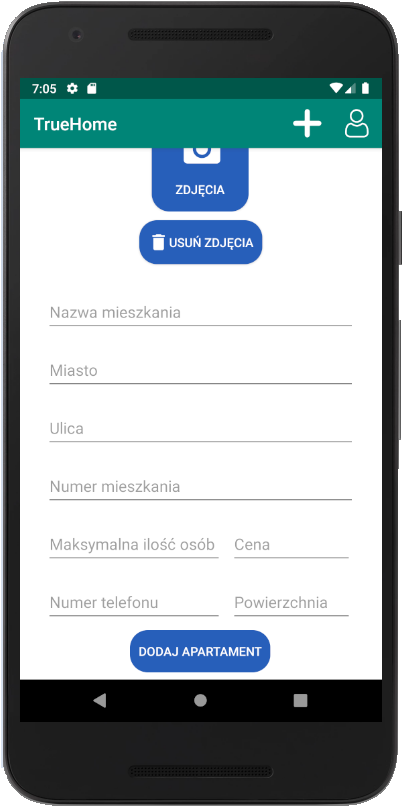
\includegraphics[width=0.45\textwidth]{aplikacja/add.png}
                    \caption{Panel dodawania nowego mieszkania}
        \end{figure}
        Aby dodać nową ofertę należy wypełnić wszystkie wymagane rubryki. Należy podać:
        \begin{itemize}
            \item nazwę mieszkania,
            \item miasto,
            \item ulicę,
            \item numer mieszkania,
            \item maksymalną ilość osób,
            \item cenę,
            \item numer telefonu,
            \item powierzchnię.
        \end{itemize}
        Przy odpowiednich typach danych sprawdzana jest poprawność tego, co jest wprowadzane. Opcjonalnie można dodać zdjęcie z aparatu lub galerii. W razie pomyłki można usunąć zdjęcia. Po wciśnięciu \texttt{DODAJ APARTAMENT} jeśli wszystkie dane są wprowadzone poprawnie to ogłoszenie zostanie wysłane do bazy danych.
      \subsubsection{Dodawanie zdjęć}
        \begin{figure}[H]
                    \centering
                    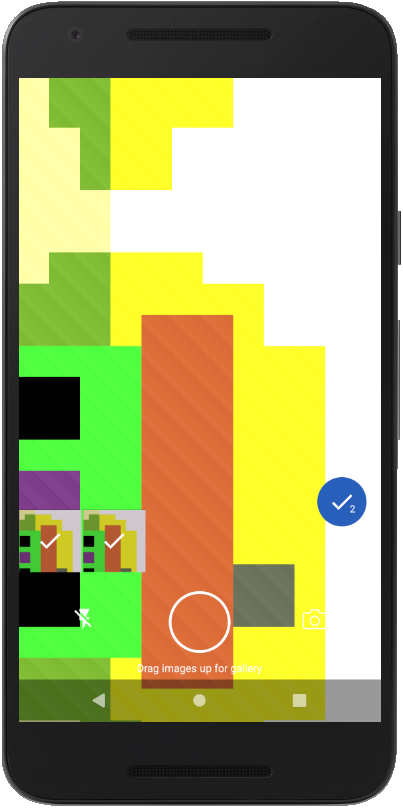
\includegraphics[width=0.45\textwidth]{aplikacja/photo.png}
                    \caption{Panel dodawania zdjęć}
        \end{figure}
        
        Użytkownik zostanie przeniesiony do tego panelu z ,,Dodawania oferty''. Można tu zrobić nowe zdjęcie lub wybrać już istniejące i dodać je do tworzonej oferty nowego mieszkania.
        
       \subsection{Szczegóły oferty}
        \begin{figure}[H]
                    \centering
                    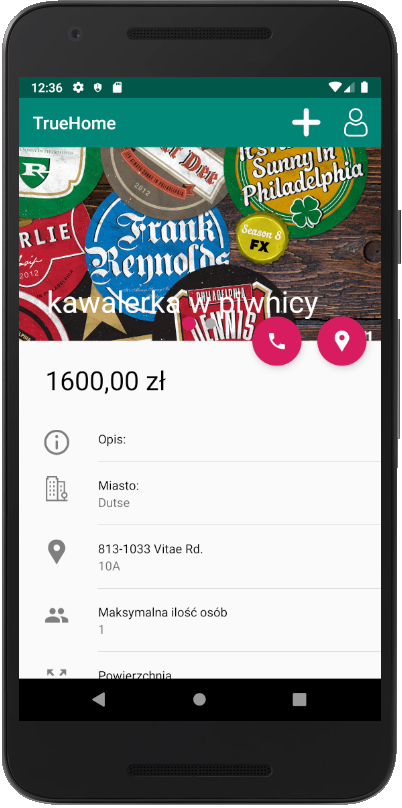
\includegraphics[width=0.45\textwidth]{aplikacja/details.png}
                    \caption{Panel szczegółów mieszkania}
        \end{figure}
        \begin{figure}[H]
                    \centering
                    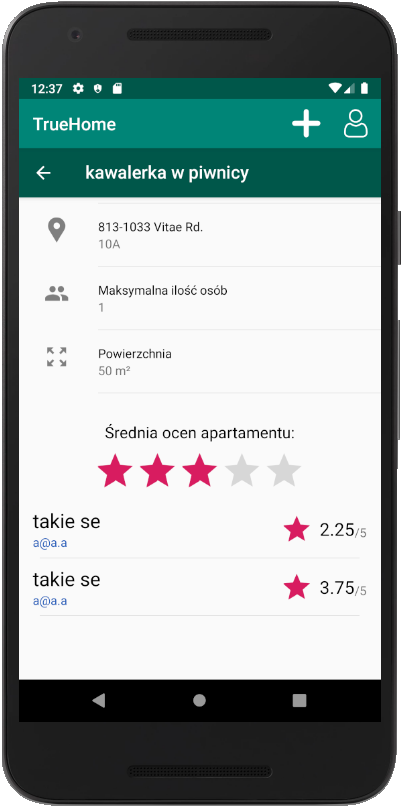
\includegraphics[width=0.45\textwidth]{aplikacja/details2.png}
                    \caption{Panel szczegółów mieszkania}
        \end{figure}
        
        W tym miejscu można przejrzeć szczegóły oferty. Wszystkie istotne dane są dostępne na tej karcie łącznie ze średnią oceną mieszkania. Istnieje możliwość przesuwania zdjęć, aby załadować następne. Po jego naciśnięciu zostanie ono powiększone. Jedną z ciekawszych możliwości jest wyświetlenie lokalizacji apartamentu na Google Maps, co bardzo ułatwia znalezienie mieszkania i ocenę okolicy. Po wciśnięciu słuchawki użytkownik przeniesiony zostanie do systemowej aplikacji służącej do dzwonienia z wprowadzonym numerem telefonu ogłoszeniodawcy.
\section{Analiza SWOT powdrożeniowa}
    \subsection{Wewnętrzne}
        \subsubsection{Mocne strony}
            \begin{itemize}
                \item System wykonany w nowoczesnych technologiach - daje to większe możliwości w tworzeniu aplikacji, w przyszłości istnieje możliwość łatwiejszej rozbudowy aplikacji. Członkowie drużyny poszerzyli swoją wiedzę na temat programowania, co może się im przydać.
                \item Kompatybilność z systemem operacyjnym Android - jest to obecnie najpopularniejszy system na platformy mobilne. Aplikacja na inne systemy może zawsze zostać stworzona dodatkowo.
                \item Zgrana ekipa - członkowie znali się już wcześniej, co pozwoliło na lepszą komunikację wewnętrzną. Dzięki temu każdy problem lub wątpliwość mogły zostać szybko skonsultowane i wyjaśnione.
                \item Dobra organizacja drużyny - dzięki dobrze wykonanej pracy lidera zespołu oraz co tygodniowym spotkaniom udało się zachować stałe tempo dodawania nowych funkcjonalności oraz jakość kodu i rozwiązań.
                \item Darmowość serwisu - aplikacja jest za darmo dla wszystkich zainteresowanych. Nie trzeba uiszczać żadnych opłat, ani nie istnieją żadne ukryte płatności.
                \item Intuicyjność aplikacji - aplikacja jest wykonana w taki sposób, aby większość osób bez czytania dodatkowych instrukcji mogła z niej sprawnie korzystać. Wszelkie błędy i komunikaty, które mogą być przekazane użytkownikowi są krótkie, jednoznaczne i proste do zrozumienia.
                \item Integracja z Google Maps - użytkownik jest w stanie w prosty sposób sprawdzić na mapie gdzie znajduje się interesujące go mieszkanie. Dzięki temu nie ma potrzeby szukania lokalizacji mieszkania poza aplikacją.
                \item Niskie koszty utrzymania aplikacji - jedynym kosztem stałym jest opłacanie serwera, jednak przy obecnym obciążeniu jest to koszt znikomy. Jako, że projekt był wykonywany na uczelnię odpadły wszelkie koszty związane z opłacaniem członków zespołu czy licencji. 
                \item Skuteczne zabezpieczenia - wykorzystane systemy autoryzacji i uwierzytelniania zapewniają bezpieczeństwo danych użytkowników.
            \end{itemize}
        
        \subsubsection{Słabe strony}
            \begin{itemize}
                \item Brak kompatybilności z innymi systemami operacyjnymi - Android zajmuje większość rynku mobilnego (zwłaszcza w Polsce), ale poprzez brak wersji na przykład iOS czy wersji webowej aplikacji, tracona jest duża część potencjalnych użytkowników na starcie.
                \item Konieczność zakładania konta, aby korzystać z wszystkich możliwości aplikacji - aby dodać mieszkanie lub je wynająć należy być zarejestrowanym. Jest to oczywista konieczność, ale nie każdy użytkownik lubi się rejestrować.
                \item Brak spójnej oprawy graficznej - w kilku miejscach oprawa nie jest do końca spójna, wynika to z tego, że aplikację robiło kilka różnych osób i oprawa graficzna nie była priorytetowa (ważniejsza była funkcjonalność).
                \item Niewielkie doświadczenie w tworzeniu dużych projektów - większość członków zespołu nigdy nie pracowało nad tak dużymi aplikacjami. Musiała się uczyć technologi i pewnych zachowań na bieżąco, co trochę spowalniało postępy pracy.
            \end{itemize}
    \subsection{Zewnętrzne}
        \subsubsection{Szanse}
            \begin{itemize}
                \item Brak takiej samej aplikacji na rynku - oczywiście, że istnieją aplikacje pozwalające wyszukiwać mieszkań, ale nie istnieje żadna nastawiona na wynajmowanie pojedynczych pokoi i ocenianie wystawiających.
                \item Rosnąca popularność systemów mobilnych - cały czas obserwuje się wzrost użytkowników smartfonów, zwłaszcza wśród ludzi młodych. Aplikacja jest skierowana głównie dla studentów, więc postawienie na systemy mobilne zwiększyło drastycznie ilość potencjalnych użytkowników.
                \item Duży popyt - każdego roku pojawia się coraz więcej młodych studentów, którzy chcieliby wynająć mieszkanie i jest to mało prawdopodobne, aby ta sytuacja w najbliższym czasie się zmieniła. 
                \item Nazwa wzbudzająca zaufanie - ,,TrueHome'', ludzie chętniej korzystają z aplikacji, które kojarzą im się im ciepło i z bezpieczeństwem.
                \item Możliwość zmonopolizowania rynku - jeśli aplikacja by się przyjęła i nie pojawiły się w najbliższym czasie konkurencyjne rozwiązania to bardzo możliwe, że jej pozycja i zasięg były na tyle duże, że byłoby bardzo ciężko jej tego statusu pozbawić.
            \end{itemize}
        \subsubsection{Zagrożenia}
            \begin{itemize}
                \item Możliwy brak zainteresowania - na początku bardzo ciężko przekonać użytkowników do stworzonego rozwiązania. Aby system działał poprawnie potrzebna jest jak największa ilość ogłoszeniodawców oraz osób chcących wynająć mieszkanie. Aby temu zapobiec należałoby zainwestować w reklamy i zachęcić czymś przyszłych użytkowników. Wszystko to wymaga sporej sumy pieniędzy, których grupa projektowa nie posiada.
                \item Brak pomysłu na marketing - z powodu, że jest to projekt uczelniany, to ten aspekt został całkowicie pominięty podczas pracy.
                \item Istnienie częściowo podobnych rozwiązań - serwisy takie jak ,,Otodom'' czy ,,OLX'' pozwalają na wystawianie ogłoszeń mieszkaniowych. Jednak nie jest to tak ukierunkowane na wynajmowanie stancji studentom jak ,,TrueHome''.
                \item Serwer może nie wytrzymać obciążenia - przy większej ilości użytkowników będzie konieczne wykupienie szybszej maszyny z większymi limitami przesyłu danych. Bez tego korzystanie z aplikacji nie będzie komfortowe.
                \item Możliwy rozpad zespołu - w każdej chwili każdy członek zespołu może przestać być studentem i tym samym nie uczestniczyć w dalszym rozwoju projektu. Zresztą po zakończeniu semestru raczej mało kto będzie dalej rozwijał aplikację.
            \end{itemize}
\end{document}